%% tags: graph network tikzImg pac pacLearning aaai aaai19 vcDimension
%% doubleArrow table tabular
\documentclass[tikz,border=2]{standalone}
\usetikzlibrary{shadows,arrows,shapes,positioning,calc,backgrounds,fit}
\newcommand{\vanish}[1]{}
\usepackage{array}
\newcommand{\calc}[1]{\mbox{$\mathcal{C}_{#1}$}}
%% \usepackage{ctable}
\pdfpageattr {/Group << /S /Transparency /I true /CS /DeviceRGB>>}
% Define the layers to draw the diagram
%
\begin{document}
%% \pgfdeclarelayer{bg}
%% \pgfdeclarelayer{fg}
%% \pgfsetlayers{bg,main,fg}
%
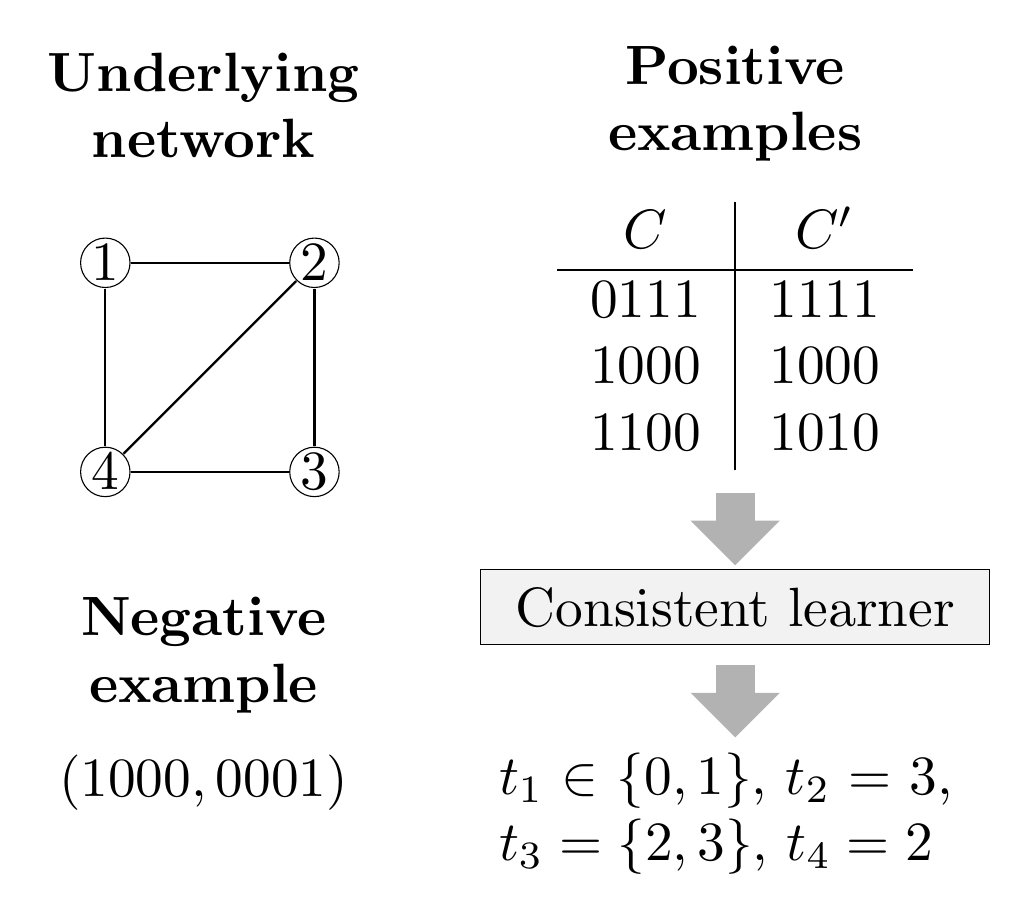
\begin{tikzpicture}
[scale=2,node distance=1cm, transform shape,
mynode/.style={shape=circle,draw=black,inner sep=.1mm},
lab/.style={fill=none},
myedge/.style={>=latex', shorten >=.0pt, shorten <=.0pt,thick},
regedge/.style={gray!60,>=triangle 90, shorten >=.4mm, shorten <=.4mm, 
line width=1.7mm,postaction={draw, line width=5mm, shorten >=3mm, -}}]
%%%%%%%%%%
%%%%% graph
%% vertices
\begin{scope}[shift={(0,0)}]
\node [above of=v1,anchor=west,shift={(0,0)},text width=2cm,align=center]
at (0,0) {\bf Underlying network};
\node (v1) [mynode] at (.5,0) {1};
\node (v2) [mynode,right=of v1] {2};
\node (v3) [mynode,below=of v2] {3};
\node (v4) [mynode,below=of v1] {4};
%% edges
\draw[myedge] (v1) -- (v2) {};
\draw[myedge] (v1) -- (v4) {};
\draw[myedge] (v2) -- (v3) {};
\draw[myedge] (v2) -- (v4) {};
\draw[myedge] (v3) -- (v4) {};
%%
\end{scope}
%% path decomposition
\begin{scope}[shift={(5,1)},node distance=.5cm]
\node (ti) [above of=v1,anchor=north,shift={(-.5,0)},text width=2cm,align=center]
at (0,0) {\bf Positive examples};
\node (pe) [anchor=north,shift={(0,-.5)}] at (ti) {
\begin{tabular}{c|c}
$C$ & $C'$ \\\hline
$0111$ & $1111$ \\
$1000$ & $1000$ \\
$1100$ & $1010$ \\
\end{tabular}
};
\draw[regedge,->] (pe.south) -- +(0,-.5);
\node (cl) [draw,rectangle,fill=gray!10,anchor=north,text
width=4cm,align=center,shift={(0,-.5cm)},text width=3cm] at
(pe.south) {Consistent learner};
\draw[regedge,->] ($(cl.south)+(0,-.1)$) -- +(0,-.5);
\node [anchor=north,shift={(0,-.8)},text width=3cm] at (cl) {
   $t_1\in\{0,1\}$, $t_2=3$, $t_3=\{2,3\}$, $t_4=2$
};
\end{scope}
%%
\begin{scope}[anchor=north west,shift={(0,-2)}]
\node (ti) [text width=2cm,align=center] {\bf Negative example};
\node [text width=2cm,align=center] at (0,-1) {$(1000,0001)$};
\end{scope}
\end{tikzpicture}
\end{document}
